\documentclass[output=paper,
colorlinks,
citecolor=brown,
newtxmath
]{langscibook}

\author{Jelena Živojinović\affiliation{University of Verona}\affiliation{UiT The Arctic University of Norway}\orcid{0000-0003-0190-0767}}
\title{Torlak clitic doubling: A cross-linguistic comparison}
\abstract{This paper examines the types of clitics and clitic placement in Torlak. This vernacular, spoken in South-Eastern Serbia, also called the Prizren-Timok variety, whose genealogical position is still debatable, requires more attention from the scientific community. In this article, I describe clitic constructions, particularly the ones of clitic doubling and word order in Torlak by presenting data collected in the area of Trgovište and comparing it to the description of Bulgarian provided in \citet{Cinque.Krapova2008}. A further crosslinguistic comparison with Serbo-Croatian, Bulgarian, and Macedonian gives an insight into the relatedness of Torlak to the two typologically different areas: a Balkan Slavic and a non-Balkan Slavic one. This is particularly interesting since Torlak has clitic doubling, which makes it similar to Bulgarian and Macedonian, but it has second-position clitics, which makes it similar to Serbo-Croatian, thereby challenging certain cross-linguistic generalizations of \citet{Boskovic2001,Boskovic2004a,Boskovic2004b,Boskovic2007,Boskovic2016}. The overall results allow us to have a clearer picture of the use of clitics in this non-standard variety.

\keywords{clitic doubling, Torlak, cross-linguistic comparison}
}


\begin{document}
\SetupAffiliations{mark style=none}
\maketitle
%%%%%%%%%%%%%%%%%%%%%%%%%%%%%%%%%%%%%%
%
%       Chapter 1
%
%%%%%%%%%%%%%%%%%%%%%%%%%%%%%%%%%%%%%%

\section{Introduction}\label{sec:zivojinovic:intro}

\ili{Torlak} is a dialect spoken in the Southern or Southeastern area of Serbia. It is often called Prizren-Timok dialect to delineate its area in Serbia, despite its distribution in closer areas in Bulgaria and Macedonia as well (\figref{fig:map}) and some minor sub-varieties in the inner Bulgaria and Romania.\footnote{The areas inhabited by the populations of Gorani and Carashovans are disputed and not always considered as \ili{Torlak} \citep{Ivic1956, Browne1993}. I will not refer to these areas in this article. The map in \figref{fig:map} does not represent the current distribution, but it is the closest one.}

%%%Fig 1 NEW POSITION
\begin{figure}[h!]
\includegraphics[width=10.5cm]{figures/map_v2.png}
\centering
\caption[Distribution of the {Torlak} dialect]{Distribution of the {Torlak} dialect (Source: \url{https://upload.wikimedia.org/wikipedia/commons/c/c1/Torlak_dialects_map_en.png})}
\label{fig:map}                     \end{figure}

What is relevant is that \ili{Torlak} contains the majority of features of the so-called Balkan Sprachbund and that there is a high level of microvariation within its area of distribution. It is often disputed by \ili{Serbian}/Croatian and \ili{Bulgarian} scholars, who claim that

\begin{enumerate}
\item \ili{Torlak} (Prizren-Timok) is a \ili{Shtokavian} or a \ili{Serbian} dialect (\citealt{Belic1905,Ivic1956,Brozovic.Ivic1988}, among others),
\item \ili{Torlak} is a \ili{Bulgarian} dialect (\citealt{Stoykov2002}, as one of the most recent studies).
\end{enumerate}

Therefore, its classification remains controversial, having some features in common with \ili{Serbo-Croatian} and some others with \ili{Bulgarian} and \ili{Macedonian}. Despite genealogical issues, this work seeks to provide a valuable contribution in the domain of typology of South \ili{Slavic} languages.

% Figure 1 fig:map
%\begin{figure}[h!]
%\includegraphics[width=10.5cm]{map_v2.png}
%\centering
%\caption[Distribution of the \ili{Torlak} dialect]{Distribution of the \ili{Torlak} dialect (Source: \url{https://upload.wikimedia.org/wikipedia/commons/c/c1/Torlak_dialects_map_en.png})}
%\label{fig:map}
%\end{figure}

In this article, I will address two important issues concerning the phenomenon of clitic doubling. On the one hand, I will represent different types of reduplication constructions by confronting \ili{Torlak} data with the framework illustrated in \citet{Cinque.Krapova2008}. On the other hand, I will deal with word order issues and clitic placement in the same structures.

The introductory  \sectref{sec:framework} will discuss the theoretical framework of clitic doubling, address the phenomenon of doubling in Balkan languages, and delineate the methodology and fieldwork conducted in South-Eastern Serbia. \sectref{sec:reduplications} will deal with different types of reduplication constructions, mainly based on \citet{Cinque.Krapova2008}, and provide evidence from the gathered data. Finally, \sectref{sec:cliticorder} will carry out a cross-linguistic comparison between \ili{Torlak} and its surrounding languages, with respect to word order.

% Section 2 : sec:framework

\section{Theoretical framework: The phenomenon of clitic doubling in a nutshell}\label{sec:framework}
The phenomenon of \textsc{clitic doubling} involves the reduplication of a verbal argument by a clitic pronoun. The doubled argument is usually a full pronoun \REF{ex:zivojinovic:1} or a DP \REF{ex:zivojinovic:2}, or in certain circumstances a CP \REF{ex:zivojinovic:3}, according to \citet[1--4]{Kallulli.Tasmowski2008}, for example:\footnote{If not indicated otherwise, examples are from \ili{Torlak}.}

% Example 1

\ea\label{ex:zivojinovic:1}
\gll Mene me boli stomak. \\
     Me.\textsc{acc} me.\textsc{cl.acc} hurts stomach \\
\glt `I have stomach ache.'
\z

% Example 2

\ea\label{ex:zivojinovic:2}
\gll Lo	vimos a Juan.\\
     Him saw.\textsc{1pl}	to Juan \\
\glt `We saw Juan.' \hfill (Rioplatense \ili{Spanish}; \citealt[32]{Jaeggli1986})\footnote{The glosses have been slightly modified compared to the original citation.}
\z

% Example 3

\ea\label{ex:zivojinovic:3}
\gll Ana	e$_i$ dinte	[\textsubscript{CP} qe Eva kishte shkuar]$_i$.
\\
     Ana.the.\textsc{nom} \textsc{3sg.cl.acc} knew {} that Eva had left\\
\glt `Ana knew (it) that Eva had left.'\hfill (\ili{Albanian}; \citealt[2]{Kallulli.Tasmowski2008})
\z

\noindent Such patterns have been widely discussed with reference to \ili{Romance} languages, see, for instance, \citet{Jaeggli1982, Jaeggli1986, Kayne1991, Sportiche1996}. Among the mentioned works, the pioneering one is surely \citet{Jaeggli1982} on Rioplatense \ili{Spanish}, a language spoken in Argentina, Uruguay, and Paraguay, along with \citet{Farkas1978} and \citet{Steriade1980} on \ili{Romanian}. Research has shown that both obligatorily demand a construction of doubling, although there are systems in other languages allowing an optional use of it.

Scholars' opinions have been divided when it comes to the formal description of clitic doubling. On the one hand, some scholars assume that clitics move from an argument position to a derived position, whereas other scholars suggest they are base-generated in their surface position as agreement markers. \citet{Sportiche1996}, however, proposes a combination of the two approaches. According to his explanation, pre-existing X$^{0}$ elements are directed to a specifier position where they license a feature F, which has to be marked off in a Spec-Head configuration, since the doubled XP* must move at LF to XP\^{} position, as indicated in \figref{ex:zivojinovic:4}.

% Figure 2: ex:zivojinovic:4

\begin{figure}
    \centering
\begin{forest}
for tree={s sep=1cm, inner sep=0, l=0}
[ClP [XP\^{}]               (
    [Cl$'$ [Cl$^0$]
        [VP [Spec]
            [VP [V$^0$] [XP$^*$]]
        ]
    ]
]
\end{forest}
    \caption{Sportiche's structural analysis of CD \citep[6]{Kallulli.Tasmowski2008}}
    \label{ex:zivojinovic:4}
\end{figure}

In addition, many more recent works deal with the phenomenon of cliticization, such as \citet{Roberts2010}, who assumes that a head X$^0$ is a category which is exclusively dominating itself and claims that clitics do not necessarily need to be part of their host, although they can, or \citet{kramer2014clitic}, who provides different criteria on how to distinguish cliticization from agreement.\footnote{\citet[54]{Roberts2010}, following \citet{Chomsky1995}, distinguishes X$^0$ from X\textsuperscript{min}; X$^0$ being a head itself and X\textsuperscript{min} consisting merely of features.} I will not insist on any specific theoretical proposal, however, further investigation on cliticization in \ili{Torlak} might shed light on how this phenomenon works in the grammar.

\subsection{Clitic doubling in Balkan languages}
\label{subsec:balkan}
Clitic doubling seems to represent an innovation in Balkan languages arisen among the languages themselves, since there is no historical attestation in either \ili{Old Church Slavonic} or \ili{Ancient Greek} \citep[9]{Kallulli.Tasmowski2008}. According to certain works, such as \citet{Lopasov1978} and \citet{Tomic2008a, Tomic2008b}, there is consistent variation across Balkan languages and even more microvariation within Balkan \ili{Slavic}. \citet{Lopasov1978} claims that western and southern areas might have strict grammatical constraints which doubling constructions are subject to, whereas northern and eastern areas might use discourse-pragmatic factors to influence CD. \citet{Tomic2008a, Tomic2008b}, despite being more focused on Balkan \ili{Slavic}, provides an illustration of the Balkan dialectal continuum. Doubling appears to show variation across a vertical North-South axis as well as across a horizontal East-West one. Moving North to South, ``along with the reduction of the distance between the clitics and the verb, the restrictions on the word classes that can be clitic doubled are relaxed'' \citep[81]{Tomic2008a}. Therefore, \ili{Serbo-Croatian} shows almost no traces of clitic doubling constructions, \ili{Torlak} exhibits a wide usage of accusative doubling and to a lesser extent dative doubling, while \ili{Macedonian} requires clitic doubling constructions obligatorily with definite direct and indirect objects. As one moves from East to West, ``along with the gradual disappearance of the rule for non-occurrence of the clitics in clause-initial position, the restrictions on the environments for clitic doubling are relaxed'' \citep[81]{Tomic2008a}.

\subsection{Data and methods}
\label{sec:dataandmethods}
The data for this study was collected in the area of Trgovište in South-Eastern Serbia. What is interesting is that the subvariety of \ili{Torlak} spoken here exhibits overt postposed articles just like \ili{Bulgarian} and \ili{Macedonian} (Balkan languages) but unlike \ili{Serbo-Croatian} (non-Balkan).\footnote{Other subvarieties of \ili{Torlak} might not exhibit overt postposed articles, such as the one analyzed in \citet{Runic2013,Runic2014}.} In fact, we find:

% Example 4

\ea\label{ex:zivojinovic:5}
\gll Vide li  ga         ribarata?\\
     saw  \textsc{q}   him.\textsc{cl.acc} fisherman.\textsc{acc.def}\\
\glt `Have you seen the fisherman?'
\z

\noindent The majority of data was collected as free production, particularly due to the age of participants, whose physical conditions did not make specific assignments possible. However, a short elicitation task was done in addition to the free production, with the use of targeted questions, in order to trigger the use of the target word order. Some of the examples can be found in \sectref{subsec:orderTorlak}. The variety of \ili{Torlak} recorded for this study is specifically relevant due to its geographical position, which is relatively close to both the \ili{Macedonian} and the \ili{Bulgarian} border. Therefore, an investigation of contact-induced phenomena might prove fruitful. However, in this article I will focus on a mere comparison of \ili{Torlak} with its bordering languages.
%%%%%%%%%%%%%%%%%%%%%%%%%%%%%%%%%%
%
%       Chapter 3
%
%%%%%%%%%%%%%%%%%%%%%%%%%%%%%%%%%%

\section{Clitic reduplication constructions}
\label{sec:reduplications}

\subsection{Relevant background: \citet{Cinque.Krapova2008}}
\label{subsec:relevantbackground}
According to \citet{Cinque.Krapova2008}, who worked on \ili{Bulgarian}, clitic doubling cannot be treated as a uniform phenomenon without first mentioning different subtypes of it. As a matter of fact, they identified four divergent subtypes within this macro group. We find:

\begin{itemize}
\item \textsc{hanging topic left dislocation} (HTLD),
\item \textsc{clitic left dislocation} (CLLD),
\item \textsc{clitic doubling proper} (CD),
\item and \textsc{clitic right dislocation} (CLRD).
\end{itemize}

CD, exemplified in \REF{ex:zivojinovic:6}, is a construction involving specific groups of predicates, as listed in \citeposst{Cinque.Krapova2008} work. For instance, they list psych and physical perception predicates with dative experiencers (e.g. \textit{lipsva mi} `I miss', lit. `miss me.\textsc{dat}'), psych and physical perception predicates with accusative experiencers (e.g. \textit{dostrašava me} `I am afraid of'), predicates with possessor datives (e.g. \textit{bučat mi ušite} `my ears ring'), predicates with possessor accusatives (e.g. \textit{vărti me ramoto} `I have a stitch in the shoulder'), predicates in the feel-like constructions (e.g. \textit{iska mi se} `I feel like'), modal predicates (e.g. \textit{slučva mi se} `it happens to me'), and predicates indicating presence or absence of something (e.g. \textit{ima} `there is', \textit{njama} `there isn’t'). Such constructions require obligatory clitic doubling, even in focus movement constructions and allow the clitic’s associate to take the stress of the utterance (as new information), to be wh-moved, to be contrastively focused and to be an indefinite quantifier.

% Example 5

\ea\label{ex:zivojinovic:6}
\gll Ne  mu          se   speše samo na Ivan.\\
     not him.\textsc{cl.dat} \textsc{refl} slept only to Ivan \\
\glt `Only Ivan didn't feel like sleeping.'
\hfill (\ili{Bulgarian})
\z

\noindent CLRD is a complementary structure to CD, but at the same time very different, according to \citet{Cinque.Krapova2008}. Namely, as in all of the constructions that will follow, doubling is not obligatory. Furthermore, there are no peculiar constraints in terms of types of predicates used, but the associate correlates with topicality and can neither be wh-moved, constitute contrastive focus, nor contain an indefinite quantifier.

% Example 7

\ea\label{ex:zivojinovic:7}
\gll Poznavam go         tova čuvstvo.\\
     know.\textsc{1sg} it.\textsc{cl.acc} this sentiment  \\
\glt `I know this sentiment.'
\hfill (\ili{Bulgarian})
\z

\noindent HTLD and CLLD are two additional complementary topic structures which mainly differ in pragmatic properties from the previous two subgroups.

Specifically, HTLD, as clearly stated in the name, creates a general context for the comment from a pragmatic point of view. From a prosodic point of view, instead, there usually is a sharper intonational break between the dislocated element on the left and the rest of the sentence. Here is an example of HTLD in \ili{Bulgarian}, taken from the corpus presented in \citet{Dzonova2004}:

% Example 8

\ea\label{ex:zivojinovic:8}
\gll Tja	 i	 bez     tova ne  moga	  da ja	        nakaram da jade.\\
     she.\textsc{nom} and without that not can.\textsc{1sg} \textsc{comp} her.\textsc{cl.acc} make.\textsc{1sg} to eat.\textsc{3sg}  \\
\glt `Her, anyway, I cannot make her eat.’ \hfill (\ili{Bulgarian})
\z

\noindent Syntactic properties are the key for distinguishing apparent cases of overlapping between HTLD and CLLD. Namely, as \citet{Cinque.Krapova2008} point out, in case of a dislocated phrase as a simple DP without overt case marking, it is necessary to take into account syntactic properties. The presence or absence of case connectivity effects, that is case matching between the dislocated element(s) and the resumptive one inside the clause, draws a clear distinction between the two subcategories. Case connectivity effects are visible in \ili{Bulgarian} but only with topicalized pronouns and, accordingly, this feature is absent in HTLD, where a topic simply bears the nominative case. Furthermore, HTLD is more likely to appear only and exclusively in root contexts and its resumptive element can be any DP.

CLLD, on the other hand, requires case connectivity effects to show up mandatorily, unlike HTLD. In addition, it appears both in root and non-root contexts and the resumptive element can only be a clitic.

% Example 9

\ea\label{ex:zivojinovic:9}
\gll Na Maria  njama    da  ì           piša       az.\\
     To Maria  \textsc{neg}.will to  her.\textsc{cl.acc}  write.\textsc{1sg}  I\\
\glt `To Maria I will not write.’
\hfill (\ili{Bulgarian})
\z

\noindent Based on these assumptions, the examples mentioned seem to represent four distinct types of doubling. More examples are to be found in \citet{Krapova.Karastaneva2002} and \citet{Cinque.Krapova2008}.

\subsection{Evidence from gathered data}                            %
\label{subsec:evidence}
Data that I am presenting here was gathered in April 2018 in the area of Trgovište, more precisely in the village Novi Glog, relatively close to the borders to Macedonia and Bulgaria. Not so surprisingly, many constructions in this dialect have a very similar, if not identical, structure to \ili{Bulgarian} and/or \ili{Macedonian}. However, my aim here is to examine whether gathered data can meet the requirements presented in \citet{Cinque.Krapova2008} and to illustrate any possible discrepancy.

I will begin with the most characteristic structure in \ili{Torlak} involving clitic doubling.

% Example 10

\ea\label{ex:zivojinovic:10}
\gll Mene   me        boli  stomak.\\
     me.\textsc{acc} me.\textsc{cl.acc} hurts stomach \\
\glt `I have a stomach ache.'
\z

\noindent This appears to be a case of CD and similar examples with tonic pronouns can be found in \ili{Bulgarian} as well. What determines the classification of the structure as the CD subtype is the use of topicalization and a specific verbal construction, involving a predicate with possessor accusative. Clitic doubling in such constructions is mandatory.
Further confirmation of CD can be found in the following examples using the types of predicates listed in \citet{Cinque.Krapova2008}.\footnote{The indicated interpretation of \REF{ex:zivojinovic:13} is not the only possible one. Another possible translation is `Marina felt better as soon as {\dots}' (`after being sick for days, she felt better'), apart from `Marina felt relief (on the soul) as soon as {\dots}'.}

\begin{itemize}
\item[i)] psych and physical perception predicates with accusative experiencers

% Beispiel 11

\ea\label{ex:zivojinovic:11}
\gll Mene   me        je  jat.\\
     me.\textsc{acc} me.\textsc{cl.acc} is  anger \\
\glt `I am angry.'
\z
\item[ii)] predicates in the feel-like constructions

% Beispiel 12

\ea\label{ex:zivojinovic:12}
\gll Na Marinu     gu         se spije.\\
     to Marina.\textsc{dat} her.\textsc{cl.dat} \textsc{refl} sleep.\textsc{3sg}\\
\glt `Marina is sleepy.'
\z

\item[iii)] predicates with possessor dative

%Beispiel 13

\ea\label{ex:zivojinovic:13}
\gll Na Marinu     gu         lkna      čim {\dots} .\\
     to Marina.\textsc{dat} her.\textsc{cl.dat} {felt.relief} {as.soon.as}\\
\glt `Marina felt relief as soon as {\dots} .'
\z

\end{itemize}

\noindent It is necessary to point out that doubling in \ili{Torlak} mainly occurs with constructions involving accusative case, whereas there are fewer examples involving dative case. In fact, specific predicates mentioned by \citet{Cinque.Krapova2008}, such as \textit{pari mi} (\textit{na ezika}) `my tongue is burning', are not grammatical in the distinct variety of \ili{Torlak} analyzed here.
CLRD occurs in \ili{Torlak} as well, being the complementary structure to CD. Indeed, example \REF{ex:zivojinovic:7} in \ili{Bulgarian} has its equivalent formation:\footnote{\ili{Torlak} does not make a distinction between proximal = V, neutral = T and distal = N articles, as \ili{Macedonian} does.}

% Example 14

\ea\label{ex:zivojinovic:14}
\gll Poznavam ga          toga čoveka.\\
     know.\textsc{1sg} him.\textsc{cl.acc} that man \\
\glt `I know that man.'
\z

\noindent Other options which are present in \ili{Bulgarian}, namely HTLD, CLLC, are lacking in \ili{Torlak}. In fact, the equivalent \ili{Torlak} examples of \REF{ex:zivojinovic:8} and \REF{ex:zivojinovic:9}, illustrated in \citet{Cinque.Krapova2008}, are ungrammatical.

% Example 15

\ea[*]
{\gll Ona     i   bez     toj  ne  moga    da gu         nakaram da jede. \\
      she.\textsc{nom} and without that not can.\textsc{1sg} \textsc{comp} her.\textsc{cl.acc} make.\textsc{1sg}    to eat\\
\glt  Intended: `And without that, I could not make her eat.'}
\z

% Example 16

\ea[*]
{\gll Na Mariju nema         da gu         pišem     ja. \\
      to Maria  there.is.not to her.\textsc{cl.acc} write.\textsc{1sg} I \\
\glt  Intended: `To Maria I do not write.'}
\z

\noindent \ili{Torlak}, therefore, only partially resembles the well-defined \ili{Bulgarian} structure.
%%%%%%%%%%%%%%%%%%%%%%%%%%%%%%%%%%%%%%%
%
%           Chapter 4
%
%%%%%%%%%%%%%%%%%%%%%%%%%%%%%%%%%%%%%%%
\section{Clitic word order}
\label{sec:cliticorder}
The following section presents issues on word order with respect to the phenomenon of clitic doubling. \sectref{subsec:assumptions} presents a theoretical part on generalizations illustrated in \citet{Boskovic2001,Boskovic2004a,Boskovic2004b,Boskovic2007,Boskovic2016}. \sectref{subsec:orderSC} and \sectref{subsec:orderBM} respectively describe all cases of word order involving cliticization in \ili{Serbo-Croatian}, and \ili{Bulgarian} and \ili{Macedonian}, whereas \sectref{subsec:orderTorlak} provides a general picture of word order in \ili{Torlak} with respect to the above-listed bordering languages.

\subsection{Relevant background: \citeauthor{Boskovic2001}'s generalizations}
\label{subsec:assumptions}
The basic assumptions for this section mainly involve crosslinguistic generalizations presented in \citet{Boskovic2001,Boskovic2004a,Boskovic2004b,Boskovic2007,Boskovic2016} and are based on the presumption that languages differ with respect to a number of syntactic and semantic phenomena depending on whether or not they have articles.

Here are the main generalizations, relevant for our word order puzzle:
\begin{enumerate}
\item Only languages with overt articles may allow clitic doubling.\label{gen:1}
\item Second position clitic systems are found only in languages without articles.\label{gen:2}
\item There is no clitic doubling with second position clitics.\label{gen:3}
\end{enumerate}

\noindent The remaining generalizations provided by Bošković are not relevant for the purpose of this article.
I will refer to these generalizations in the following sections, by illustrating clitic constructions involving auxiliary, pronominal, and other types (such as question clitics, e.g. \textit{li}) of clitics in \ili{Torlak} and its surrounding languages.

\subsection{Word order in Serbo-Croatian}
\label{subsec:orderSC}
\ili{Serbo-Croatian} has Wackernagel position clitics, according to \citet[217]{Franks.King2000}, whereas according to \citet{Boskovic2001} and \citet{Radanovic-Kocic1988,Radanovic-Kocic1996} SC clitics occur in the second position of their intonational phrase. The following examples seem to merge these two approaches:

% Example 17

\ea\label{ex:zivojinovic:17}
\gll Olga nam        nešto     dovikuje.\\
     Olga us.\textsc{cl.dat}  something shout.out.\textsc{3sg}\\
\glt `Olga is shouting out to us.'
\hfill (SC)
\z

% Example 18

\ea\label{ex:zivojinovic:18}
\gll Nešto     nam       dovikuje.\\
     something us.\textsc{cl.dat} shout.out.\textsc{3sg}\\
\glt `S/he is shouting out to us.'
\hfill (SC; \citealt[105]{Radanovic-Kocic1988})
\z

\noindent However, \citet[219]{Franks.King2000} further specify that ``in SC clitics are traditionally described as being able to fall after either the first prosodic or syntactic phrase''. In case of the presence of multiple clitics, the internal organization of the clitic cluster is the following:\footnote{\textit{Je} is an exceptional, yet problematic clitic in SC. It can occur as a \textsc{3sg} copula/auxiliary but also as a question clitic. Further details can be found in \citet{Franks2017} and \citet{Zivojinovicinpreparation}, among others.}

\begin{itemize}
\item \textsc{li} (\textsc{q}) $>$ \textsc{aux} $>$ \textsc{dat} $>$ \textsc{acc} $>$ \textsc{gen} $>$ \textsc{se} (\textsc{refl}) $>$ \textsc{je}
(be.\textsc{3sg})
\end{itemize}

\noindent In fact, we find the following examples of a maximal projection as in \REF{ex:zivojinovic:19} or a prosodic word as in \REF{ex:zivojinovic:20}.

% Example 19

\ea\label{ex:zivojinovic:19}
\gll\minsp{[} Ovu  zanimljivu  knjigu] sam      joj         pročitao.\\
    {} this  interesting book    \textsc{aux.1sg}  her.\textsc{cl.dat} read \\
\glt `I read this interesting book to her.'
\hfill (SC; \citealt[219]{Franks.King2000})
\z


% Example 20

\ea\label{ex:zivojinovic:20}
\gll\minsp{[} Anina im          sestra] nudi      čokoladu.           \\
    {} Ana’s  them.\textsc{cl.dat} sister  offer.\textsc{3sg} chocolate \\
\glt `Ana’s sister is offering them chocolate.'
\hfill (SC; \citealt[414]{Progovac1996})
\z

\noindent Second position clitics are to be found in different types of configurations: in verb-initial clauses as in \REF{ex:zivojinovic:21} and with a clitic in first position as in \REF{ex:zivojinovic:22}.

% Example 21

\ea\label{ex:zivojinovic:21}
\gll Dade      mi      ga      Nena.           \\
     gave.\textsc{3sg} me.\textsc{dat}  it.\textsc{acc}  Nena \\
\glt `Nena gave it to me.'
\hfill (SC; \citealt[222]{Franks.King2000})
\z

% Example 22

\ea\label{ex:zivojinovic:22}
\gll Je li on došao?\\
     \textsc{aux.3sg} \textsc{q} he come\\
\glt `Has he come?'
\hfill (SC; \citealt[46]{Radanovic-Kocic1988})
\z



\noindent The clitic-first configuration in \REF{ex:zivojinovic:21} illustrates one of the two possible exceptions to the second-position placement. Namely, clitics as unstressed particles cannot occur in the first position. However, the clitic \textit{je} has a stressed counterpart, making it a non-clitic, according to \citet[226]{Franks.King2000}. It is followed by the question clitic \textit{li}, which occurs in the typical second position.

Another apparent exception to the second-position is illustrated in the following example:

% Example 23

\ea\label{ex:zivojinovic:23}
\gll\minsp{[} Ono najvažnije]    dade     mi        mama.       \\
    {} that \textsc{sup}.important gave.\textsc{3sg} me.\textsc{cl.dat} mum \\
\glt `The essential thing I received from mum.'
\hfill (SC)
\z

\noindent Despite the apparent violation of the second position placement claimed by both \citet{Franks.King2000} on the one hand and \citet{Boskovic2001} and \citet{Radanovic-Kocic1988} on the other, this example requires a specific intonation and a separation of the initial constituent from the remaining part of the sentence. In this way, this constituent does not violate the second position placement.

This section concludes that there is no evidence for SC to have any other configurations than second-position placement of clitics.

\subsection{Word order in Bulgarian and Macedonian}
\label{subsec:orderBM}
Despite being typologically related, \ili{Bulgarian} and \ili{Macedonian} differ with respect to clitic doubling. Namely, they both allow CD but relate to it in a very different manner. \ili{Macedonian} has obligatory clitic doubling with definite direct and indirect objects, whereas CD in \ili{Bulgarian} is optional. In fact, as already mentioned above, it is associated with topicality and specificity \citep{Sportiche1996,Cinque.Krapova2008}.

In \ili{Bulgarian}, clitics precede finite verbs (except when the finite verb is in the first position). This means that clitics can be placed in any position in the sentence, except for the first one; see \REF{ex:zivojinovic:24}.

% Example 24

\ea\label{ex:zivojinovic:24}
\gll Vera mi        go         dade.           \\
     Vera me.\textsc{cl.dat} it.\textsc{cl.acc} gave.\textsc{3sg}\\
\glt `Vera gave it to me.'
\hfill (\ili{Bulgarian}; \citealt[234]{Franks.King2000})
\z

% Example 25

\ea\label{ex:zivojinovic:25}
\gll Koj kakvo ti          e    kazal?                                    \\
     who what  you.\textsc{cl.dat}  \textsc{aux}  told\\
\glt `Who told you that?'
\hfill (\ili{Bulgarian}; \citealt[461]{rudin1988multiple})
\z

\noindent A slightly different configuration can be found in \ili{Macedonian}. Namely, clitics always precede finite verbs and there are no further restrictions. In fact, unlike \ili{Serbo-Croatian} and \ili{Bulgarian}, \ili{Macedonian} allows first-position clitics as well.

% Example 26

\ea\label{ex:zivojinovic:26}
\gll Im           rekov     oti čovekot     te         videl. \\
     them.\textsc{cl.dat}  told.\textsc{1sg}  \textsc{comp}   person.\textsc{def}  you.\textsc{cl.acc} saw\\
\glt `I told them that the person saw you.'\\
\hfill (\ili{Macedonian}; \citealt[236]{Franks.King2000})
\z

\noindent Let us now examine the word order in \ili{Torlak}.

%%% Subsection 3.4

\subsection{Word order in Torlak}
\label{subsec:orderTorlak}

When it comes to the variation in clitic placement, \ili{Torlak} surely stands somewhere in between the above-mentioned possible scenarios. Because \ili{Torlak} allows clitic doubling, as exemplified in \REF{ex:zivojinovic:27}, one might be tempted to assume that word order in clitic constructions might resemble either \ili{Bulgarian} or \ili{Macedonian}. But let us check some examples and counter-examples:

% Example 27

\ea\label{ex:zivojinovic:27}
\gll Ti      me         mene    čekaš?\\
     you.\textsc{nom} me.\textsc{cl.acc}  me.\textsc{acc}  wait.\textsc{2sg} \\
\glt `Are you waiting for me?'
\z

\noindent Example \REF{ex:zivojinovic:28} illustrates the use of a clitic-first construction. Just as in SC, the first-position \textit{je} is stressed and may function as an auxiliary or a copula, or be part of a complex question marker (ex. \ref{ex:zivojinovic:28}). Therefore, it is not a regular clitic, but is followed by a regular question clitic \textit{li} (shortened \textit{l'}) in the second position.

% Example 28

\ea\label{ex:zivojinovic:28}
\gll Je l’  me         mene    čekaš?\\
     be.\textsc{3sg} \textsc{q} me.\textsc{cl.acc}  me.\textsc{acc}  wait.\textsc{2sg} \\
\glt `Are you waiting for me?'
\z

% Example 29

\ea\label{ex:zivojinovic:29}
\gll Mene    li  me         čekaš?\\
     me.\textsc{acc}  \textsc{q}   me.\textsc{cl.acc}  wait.\textsc{2sg} \\
\glt `Are you waiting for me?'
\z

% Example 30

\ea\label{ex:zivojinovic:30}
\gll Ja ga         poznavam Milovana.\\
     I  him.\textsc{cl.acc} know.\textsc{1sg}     Milovan \\
\glt `I know Milovan.'
\z

\noindent Unlike examples \REF{ex:zivojinovic:29} and \REF{ex:zivojinovic:30}, example \REF{ex:zivojinovic:31} displays a configuration involving a verb-initial construction. Just as in previous cases, the clitic appears in the second position (as in example \REF{ex:zivojinovic:28}).


% Example 31

\ea\label{ex:zivojinovic:31}
\gll Poznavam ga          Milovana.\\
     know.\textsc{1sg}    him.\textsc{cl.acc}  Milovan \\
\glt `I know Milovan.'
\z

\noindent The following \ili{Torlak} examples display different configurations suitable for \ili{Macedonian}, \ili{Bulgarian} and SC:

% Example 32


\ea[]{\label{ex:zivojinovic:32}
\gll Milovana  ga          poznavam.\\
     Milovan   him.\textsc{cl.acc}  know.\textsc{1sg} \\
\glt `I know Milovan.'}
\z

% Example 33

\ea[*]
{\gll Ga         poznavam Milovana.\\
     him.\textsc{cl.acc}  know.\textsc{1sg}     Milovan\\\label{ex:zivojinovic:33}
\glt Intended: `I know Milovan.'}
\z

% Example 34

\ea[]{\label{ex:zivojinovic:34}
\gll Odamna            ga          upozna Milovana.\\
    long.time.ago   him.\textsc{cl.acc}  met.\textsc{1sg}    Milovan \\
\glt `I met Milovan a long time ago.'}
\z

% Example 35

\ea[]{\label{ex:zivojinovic:35}
\gll Odamna ga Milovana upozna. \\
   long.time.ago   him.\textsc{cl.acc}  Milovan   met.\textsc{1sg} \\
\glt `I met Milovan a long time ago.'}
\z

% Example 36

\ea[]{\label{ex:zivojinovic:36}
\gll Milovana ga         upozna odamna.\\
     Milovan  him.\textsc{cl.acc} met.\textsc{1sg}    long.time.ago\\
\glt `I met Milovan a long time ago.'}
\z

% Example 37

\ea[]{\label{ex:zivojinovic:37}
\gll Milovana ga         odamna                 upozna. \\
     Milovan  him.\textsc{cl.acc} long.time.ago met.\textsc{1sg} \\
\glt `I met Milovan a long time ago.'}
\z

% Example 38

\ea[*]
{\gll Odamna            Milovana   ga         upozna.\\
    long.time.ago  Milovan    him.\textsc{cl.acc} met.\textsc{1sg} \\\label{ex:zivojinovic:38}
\glt Intended: `I met Milovan a long time ago.'
}
\z

% Example 39

\ea[]{\label{ex:zivojinovic:39}
\gll Toga ga         čoveka poznavam. \\
     that him.\textsc{cl.acc} man    know.\textsc{1sg} \\
\glt `I know that man.'}
\z

\noindent It emerges from the above-listed examples that configurations which are allowed in both \ili{Bulgarian} (see \REF{ex:zivojinovic:38} where the clitic is in the third position and precedes the main verbs) and \ili{Macedonian} (see \REF{ex:zivojinovic:33}, clitic-first construction) are not acceptable in \ili{Torlak}. On the other hand, as examples \REF{ex:zivojinovic:35} and \REF{ex:zivojinovic:37} show, \ili{Torlak} allows non-verb-adjacent clitics, unlike \ili{Bulgarian} and \ili{Macedonian}. Just as \ili{Serbo-Croatian}, it supports the use of clitics after the first prosodic word (example \REF{ex:zivojinovic:39}), following \citet{Boskovic2001} and \citet{Radanovic-Kocic1988}.

How does such evidence relate to Bošković’s generalizations? This sub-variety of \ili{Torlak} seems to fit into Bošković’s Generalization \ref{gen:1}, mentioned above, but not into the Generalizations \ref{gen:2} and \ref{gen:3}. However, the postposition of the article does not seem to be widespread all across the distribution of \ili{Torlak}. In fact, the \ili{Torlak} (Prizren-Timok) data presented in \citet{Runic2014} and gathered in the Timok area shows the use of clitic doubling but no overt articles, fitting into Generalizations \ref{gen:2} and \ref{gen:3}, but not \ref{gen:1}.
%%%%%%%%%%%%%%%%%%%%%%%%%%%%%%%%%%%
%
%           Chapter 4
%
%%%%%%%%%%%%%%%%%%%%%%%%%%%%%%%%%%%
\section{Conclusion}
\label{sec:conclusion}

The theory displayed in \citet{Cinque.Krapova2008} satisfactorily describes the phenomenon of clitic doubling in \ili{Bulgarian} by identifying four subtypes:
\begin{itemize}
\item clitic doubling proper,
\item clitic right dislocation,
\item hanging topic right dislocation,
\item and clitic left dislocation.
\end{itemize}
However, this branching does not seem to adequately work for \ili{Torlak}, which adopts the canonical structure of clitic doubling mainly with tonic pronouns, but also with DPs.

Concerning word order, it emerges that, although \ili{Torlak} allows clitic doubling as \ili{Bulgarian} and \ili{Macedonian}, it is closer to \ili{Serbo-Croatian}, which allows only one constituent to precede the clitic cluster. This specific variety, having post-positioned overt articles, is incompatible with Bošković’s generalizations.

% ABBREVIATIONS

\section*{Abbreviations}

\begin{tabularx}{.45\textwidth}{lX}
\textsc{1}&first person\\
\textsc{3}&third person\\
\textsc{acc}&accusative case\\
\textsc{aux}&auxiliary\\
\textsc{cl}&clitic\\
\textsc{dat}&dative case\\
\textsc{comp}&complementizer\\
\end{tabularx}
\begin{tabularx}{.45\textwidth}{lX}
\textsc{def}&definite article\\
\textsc{neg}&negation\\
\textsc{nom}&nominative case\\
\textsc{refl}&reflexive marker\\
\textsc{sg}&singular\\
\textsc{pl}&plural\\
\textsc{q}&question particle\\
\end{tabularx}

% ACKNOWLEDGEMENTS

\section*{Acknowledgements}

I would like to thank the audience of the FDSL 13 in Göttingen and two anonymous reviewers for valuable feedback, as well as the editors of this volume. Lastly, I would like to express my gratitude to all the speakers who participated in this study, particularly my great-grandmother, Petkana. I dedicate this article to her memory.

\sloppy
\printbibliography[heading=subbibliography,notkeyword=this]
\end{document}
